% Kompiuterijos katedros šablonas
% Template of Department of Computer Science II
% Versija 1.0 2015 m. kovas [ March, 2015]

\documentclass[a4paper,12pt,fleqn]{article}
\usepackage[unicode,colorlinks=false]{hyperref}


\usepackage[utf8x]{inputenc}
%

\usepackage[L7x]{fontenc}
\usepackage{times}
\usepackage{ucs}

 %package to switch the language
\usepackage{etoolbox}

  %set up of the page margins
\usepackage[top=2cm, bottom=2cm, left=3cm, right=1.5cm]{geometry}

 %1.1 line spacing
\linespread{1.1}


  %page numbering at the right side
\usepackage{fancyhdr}
\pagestyle{fancyplain}
\fancyhf{}
\renewcommand{\headrulewidth}{0pt} 
\fancyhfoffset[RO]{0cm}

  %to number at the bottom (exchange lines to number at the top)
\rfoot{\thepage}
  %\rhead{\thepage} %

% \usepackage[usenames,dvipsnames]{pstricks}
\urlstyle{same}
\hypersetup{
%  citecolor=Blue,
%  linkcolor=Blue,
%  urlcolor=Blue
pdfborder={0 0 0 }
}

 %for includegraphics
\usepackage{graphicx}



\usepackage[toc,page]{appendix}


\usepackage{caption}

 %for source codes
\usepackage{listings}
\lstset{commentstyle=\color{red},xleftmargin=10pt, framexleftmargin=6pt, numbersep=1mm, frame=single, numbers=left,numberstyle=\footnotesize,extendedchars=\true, inputencoding=utf8x,basicstyle=\footnotesize,extendedchars=true,
 keywordstyle=\color{black}\bfseries, breaklines=true, breakautoindent=true,framesep=8pt,linewidth=0.95\textwidth
}

 %for algorithms
\usepackage{algorithm}
\usepackage{algorithmic}
 %instead of the above two packages we can use algorithms2e
 %\usepackage[boxed,linesnumbered,vlined,slide]{algorithm2e}

 %special symbols
\usepackage{amsfonts}
\usepackage{amssymb}
\usepackage{amsmath}

 %for theorem like environments
\usepackage{amsthm}

 \usepackage{datetime}
 \renewcommand{\dateseparator}{--}


% SI system units
\usepackage{siunitx}
\sisetup{detect-all}
% Problem with fonts \SI{x.xx}{\micro\metre}, solved with updmap-sys --enable Map=utm.map
\renewcommand{\sfdefault}{uhv}
\renewcommand{\rmdefault}{utm}
\renewcommand{\ttdefault}{ucr}

% List management (itemize, etc.)
\usepackage{enumitem}

\newcommand*{\urlw}[1]{\href{#1}%
            {\nolinkurl{#1}}}
    

\numberwithin{equation}{section}


\newtoggle{inLithuanian}
 %If the report is in Lithuanian, it is set to true; otherwise, change to false
\settoggle{inLithuanian}{true}

%create file preface.tex for the preface text
%if preface is needed set to true
\newtoggle{needPreface}
\settoggle{needPreface}{false}

\newtoggle{signaturesOnTitlePage}
\settoggle{signaturesOnTitlePage}{true}


\theoremstyle{definition}
\newtheorem{definition}{\keyWordDefinition}
\newtheorem{example}{\keyWordExample}
\def\QED{\unskip\nobreak\hfill\kern5pt$\Box$}

\iftoggle{inLithuanian}{
%\usepackage[L7x]{fontenc}
\usepackage[english,lithuanian]{babel}

\newcommand{\todayiso}{\the\year \dateseparator \twodigit\month \dateseparator \twodigit\day}


\renewcommand{\today}{\number\year\space m. \space \ifcase\month\or
  sausio\or vasario\or kovo\or balandžio\or gegužės\or birželio\or
  liepos\or rugpjūčio\or rugsėjo\or spalio\or lapkričio\or
  gruodžio\fi
  \space\number\day\space d.}


 \usepackage{tocloft}
 \renewcommand\cftsecaftersnum{.} 
 \renewcommand\cftsubsecaftersnum{.} 
 \renewcommand\cftsubsubsecaftersnum{.}

 \usepackage{VUMIFKK}

 \DeclareCaptionLabelFormat{captionlt}{#2 #1}
   %smth is not fine with algorithms 
 \DeclareCaptionLabelFormat{captionltalg}{#2 #1 algoritmas}

 \usepackage{indentfirst}
 \renewcommand{\appendixtocname}{Priedai}
 \renewcommand{\appendixpagename}{Priedai}
 \renewcommand{\contentsname}{Turinys} 

 \renewcommand{\lstlistingname}{išeities kodas}
 \renewcommand{\figurename}{pav}
 \renewcommand{\tablename}{lentelė}


 \captionsetup*[lstlisting]{   
 labelsep=period,labelformat=captionlt
 }
 \captionsetup*[figure]{   
% labelsep=period,
 labelsep=space, %babel redefines pav to pav.
 labelformat=captionlt
 }
 \captionsetup*[table]{   
  labelsep=period,
  labelformat=captionlt
 }
 \renewcommand{\algorithmicrequire}{\textbf{Įvestis:}}
 \renewcommand{\algorithmicensure}{\textbf{Išvestis:}}

 \captionsetup*[algorithm]{   
 labelsep=period,labelformat=captionltalg
 }

\renewcommand{\thmhead}[3]{#2 #1#3}

}
{
%\usepackage[OT1,T1]{fontenc}
%\usepackage[L7x]{fontenc}



\usepackage[english]{babel}
\newcommand{\todayiso}{\twodigit\month \dateseparator \twodigit\day \dateseparator \the\year}
 \captionsetup*[algorithm]{   
 labelsep=period
 }
\captionsetup*[lstlisting]{   
 labelsep=period
 }
 \captionsetup*[figure]{   
 labelsep=period
 }
 \captionsetup*[table]{   
 labelsep=period
 }


}

%some kywords
 \def\keywordAbstract{\iftoggle{inLithuanian}{Santrauka}{Abstract}}
 \def\keywordAbstractOther{\iftoggle{inLithuanian}{Summary}{Santrauka}}
 \def\keyWordIntroduction{\iftoggle{inLithuanian}{Įvadas}{Introduction}}
 \def\keyWordConclusions{\iftoggle{inLithuanian}{Išvados ir rekomendacijos}{Conclusions and Recommendations}}

 \def\keyWordPreface{\iftoggle{inLithuanian}{Pratarmė}{Preface}}
 \def\keyWordAppendice{\iftoggle{inLithuanian}{Priedas}{Appendix}}
 \def\keyWordSignature{\iftoggle{inLithuanian}{parašas}{signature}}
 \def\keyWordDefinition{\iftoggle{inLithuanian}{apibrėžimas}{Definition}}
 \def\keyWordExample{\iftoggle{inLithuanian}{pavyzdys}{Example}}

\newcommand{\bothabstracts}[3]{
\setcounter{secnumdepth}{0}
\newpage
\hspace{2cm}
{\centering{\section{\keywordAbstract}}}

#1
\newpage
\hspace{2cm}
{\centering \section{\keywordAbstractOther}}

\begin{center}{\textbf{#2} }\end{center}

 #3
\setcounter{secnumdepth}{3}
}

 %non-numbered sections: #1 param: for labeling sec:#1, #2 -section title
\newcommand{\sectionWithoutNumber}[2]{\newpage
%\hspace{2cm}
\section*{#1}
\label{sec:#2}
\addcontentsline{toc}{section}{\nameref{sec:#2}}%{#3}
 }



\newcommand{\referenceSources}[1]{
\newpage
\cleardoublepage
\phantomsection
\iftoggle{inLithuanian}{
 \renewcommand{\refname}{Literatūros šaltiniai}

 \addcontentsline{toc}{section}{Literatūros šaltiniai}
 \markboth{\refname}{Literatūros šaltiniai}
 }
{

\addcontentsline{toc}{section}{References}
\markboth{References}{References}
}

\bibliographystyle{plain}
\bibliography{#1}
}



 \newcommand\authorsignature[1]{
\begin{flushright}
 \begin{minipage}[b]{0.45\textwidth}
  \centering
  \rule{\textwidth}{0.5pt}\\
   #1
  \end{minipage}
\end{flushright}
 }




 \newcommand\authorsignatures[5]{%
   \vspace{1cm}
   \authorsignature{#1}
   \ifstrequal{#2}{}{}{\vspace{0.3cm}
     \authorsignature{#2}
     \ifstrequal{#3}{}{}{\vspace{0.3cm}
      \authorsignature{#3}
      \ifstrequal{#4}{}{}{\vspace{0.3cm}
        \authorsignature{#4}
        \ifstrequal{#5}{}{}{\vspace{0.3cm}
         \authorsignature{#5}       
        }
      }
    }
} 
}

\newcommand{\authortitle}{
\iftoggle{signaturesOnTitlePage}{
\tiny{\keyWordSignature}
}{}
}

\newcommand{\depttitlepage}[8]
{
\thispagestyle{empty}
\begin{center}


\includegraphics[width=2cm]{jb_VU_zenklas}

%\vspace{-1cm}

\iftoggle{inLithuanian}
{ 
  VILNIAUS UNIVERSITETAS\\
  MATEMATIKOS IR INFORMATIKOS FAKULTETAS\\
  INFORMATIKOS INSTITUTAS\\
  KOMPIUTERINIO IR DUOMENŲ MODELIAVIMO KATEDRA
}
{
  VILNIUS UNIVERSITY \\
  FACULTY OF MATHEMATICS AND INFORMATICS \\
  INSTITUTE OF COMPUTER SCIENCE\\
  DEPARTMENT OF COMPUTATIONAL AND DATA MODELING
}

\vspace{5cm}

#1\\
\vspace{0.5cm}
\textbf{\Large #2}
\end{center}

\vspace{5cm}


\hspace{0.5\textwidth}
\begin{minipage}{0.4\textwidth}
 \begin{flushleft} 
\iftoggle{inLithuanian}
{
 \ifstrequal{#3}{}{}{Atliko:\\[5pt]}
}
{
\ifstrequal{#3}{}{}{Done by:\\[5pt]}
}

%\noindent
\begin{tabular}{@{}lr}%\setlength\tabcolsep{0pt}
\ifstrequal{#3}{}{}{#3&\hspace{2cm}\authortitle\\[5pt]}
\ifstrequal{#4}{}{}{#4&\authortitle\\[5pt]}
\ifstrequal{#5}{}{}{#5&\authortitle\\[5pt]}
\ifstrequal{#6}{}{}{#6&\authortitle\\[5pt]}
\ifstrequal{#7}{}{}{#7&\authortitle\\}
\end{tabular}

\end{flushleft}

\end{minipage}

\vspace{0.5cm}
\hspace{0.5\textwidth}
\begin{minipage}{0.4\textwidth}
 \begin{flushleft} 

\ifstrequal{#8}{}{}
{

\iftoggle{inLithuanian}
{
Vadovas:
}
{
Supervisor:
}

#8

}

\end{flushleft}

\end{minipage}


\vfill

\begin{center}
Vilnius\\
\the\year
\end{center}

\iftoggle{needPreface}{
 \sectionWithoutNumber{\keyWordPreface}{preface}
Pratarmės (Preface) informacija


\iftoggle{inLithuanian}
{
\vspace{\baselineskip}\hfill
\today
}
{
 \vspace{\baselineskip}\hfill \today
}

 \vspace{5cm}

\iftoggle{signaturesOnTitlePage}{}
{
\authorsignatures{#3}{#4}{#5}{#6}{#7}
}
}{}
\newpage
}


\begin{document}
 % #1 -report type, #2 - title, #3-7 students, #8 - supervisor
 \depttitlepage{Bakalauro darbas}{Saugus pažeidžiamumų skaitytuvas sistemų auditavimui}{Jonas Gavėnavičius } 
 {}{}{}{}% students 2-5
 {Lektorius Virgilijus Krinickij}

\tableofcontents


%keywords and notations if needed
\sectionWithoutNumber{Sutartinis terminų žodynas}{FTP}{
	\begin{itemize}
		\item FTP - \textit{File trasnfer protocol} Failų perkėlimo protokolas, protokolas leidžiantis perkelti duomenis iš vienos sitemos į kitą\cite{postel1985file}.
		\item MITM - \textit{Man in the middle} - „Žmogaus viduryje“ ataka – kibernetinės atakos tipas, kai puolėjas perima bendravimą tarp serverio ir kliento\cite{callegati2009man}.
		\item 	Buf{}fer overflow – viena iš potencialių rizikų, kai dėl per didelio kiekio duomenų informacija yra perrašoma gretimuose atminties blokuose\cite{cowan1998stackguard}.
		\item 	SSH - \textit{Secure Shell} – tinklo protokolas, kuris leidžia vartotojui saugiai pasiekti sistemą per nesaugų tinklą \cite{ylonen2006secure}.
		\item Framework - karkasas, į kurį įeina kelios (ar daugiau) programinės įrangos.
		\item 	NASL - \textit{Nessus Attack Scripting Language} – paprasta kalba, kuri skirta aprašyti atskiroms grėsmėms ir galimoms atakoms.
		\item IDS - \textit{Intrusion detection system} – sistema, skirta aktyviam saugumui, ji gali aptikti išpuolį realiu laiku\cite{sakri2004intrusion}.
		\item IPS - \textit{Intrusion prevention system} – \textit{IDS} papildymas, kuris gali aptikti įsilaužimą ir jį sustabdyti\cite{sakri2004intrusion}.
		\item HTTP - \textit{HyperText Transfer Protocol} – informacijos priėmimo ir perdavimo protokolas\cite{fielding1999hypertext}.
		\item Daemon – programa, kuri veikia fone ir nėra valdoma vartotojo, bet laukia specifinio įvykio ar salygos suveikti.
		\item Slaptas įėjimas – kodo dalis, kuri leidžia atakuotojui į sistemą patekti nepastebėtam.
		\item Kenkėjiška programinė įranga – bendras pavadinimas tokiai programinei įrangai, kuri yra kenkėjiška ir patenka į sistemą be vartotojo leidimo\cite{grewal2017hybrid}.
		\item SQL injekcija – vienas iš kibernetinės atakos tipų, kai vartotojo įvestis internetinėje svetainėje yra sumanipuliuojama taip, kad ji padarytų daugiau nei buvo planuota, paveiktų duomenų bazę ir joje įgyvendintų užklausą\cite{mcwhirter2018sql}.
		\item Fišingas – būdas skirtas pavogti privačią informaciją apsimetant tam tikru tiekėju.
	\end{itemize}
}

 %both abstracts
\bothabstracts{Šiais laikais, kai pasaulis tampa vis labiau ir labiau skaitmenizuotas, iškyla opi problema – kibernetinė sauga. Vis daugiau pavyzdžių kasdieniame gyvenime matome, kai įsibraunama į sistemas, kurios yra
išnaudojamos finansiniais ar kitais tikslais. Dėl to nukenčia tiekėjai prarasdami savo reputaciją ir kapitalą, tų sistemų
vartotojai, kai jų privati informacija pavogiama ir paviešinama. Niekas nėra saugus nuo tokių situacijų. Todėl valstybės, įmonės ir korporacijos vis daugiau investuoja
į kibernetinę saugą. Kibernetinė sauga tampa vis dažnesne diskusija visuomenėje, vis daugiau
dėmesio ir resursų skiriama būtent kibernetinei saugai, stengiamasi užkirsti kelią situacijoms, kurios atneštų žalą vartotojams, įmonėms ar net šalims. Kuriami
įrankiai, kurie padeda apsisaugoti nuo tokių situacijų, analizuoja sistemas ir randa jų spragas. Įrankiai pritaiko įvairias technologijas ar metodus,
kurie perspėja apie galimą arba vykstančią ataką prieš sistemą, ištaiso rastas sistemos spragas, kol jų nerado asmenys, kurie jomis pasinaudotų.}%tex-file of abstract in original language
{Secure Vulnerability Scanner for System Auditing} %if work is in LT this title should be in English
{Nowadays, as the world becomes more and more digitized, cyber security is a major issue. As a result, states, businesses and corporations are increasingly investing in cybersecurity. Ef{}forts are being made to prevent situations that could harm consumers, businesses or even countries. Tools are developed to help prevent such situations, analyze systems and identify gaps.

The purpose of this work is to create a secure vulnerability scanning tool that can safely scan the Internet
site, its system and its files, and provide information about the scan results.

This paper introduces a secure vulnerability scanner for auditing systems and websites..
It also presents an analysis of related work that reveals best practices of other scanners and their implementation in this scanner.
In addition, the methods of vulnerability and bug analysis, their analysis and implementation in the scanner are presented.
The scanner was developed using C\# programming language, .NET Core and Angular frameworks, Docker container technology, Microsoft SQL database.
A vulnerability scanner can detect external system vulnerabilities and malicious software in web site files.
It is also capable of detecting whether a website is safe to visit, its open directories or pages that users should not have access to.
Scanner security is ensured by container technology, which ensures that malware does not enter the scanner system when scanning website files or performing other scanning operations.}%tex-file of abstract in other language


 %Introduction section: label is sec:intro
\sectionWithoutNumber{\keyWordIntroduction}{intro}
Šiame darbe kuriamas saugus įrankis, kuris neišduotų savo serverio vietos ir vartotojai pasinaudoję juo galėtų gauti išsamią informaciją apie jų internetinėje svetainėje egzistuojančias spragas
bei pažeidžiamumus ar modifikuotus failus. Darbo tikslas – sukurti saugų pažeidžiamumų skenavimo įrankį, kuris pasileistų iš tam tikros VPN technologija slepiamos vietos, skenuotų internetinę
svetainę bei jos failus, aptiktų pažeidžiamumus ar modifikuotus failus, ir pateiktų klientui informaciją apie skenavimo rezultatus. Siekiant, kad darbas būtų paklausus ir veiksmingas, keliami šie
darbo uždaviniai:
\begin{enumerate}
	\item Apžvelgti egzistuojančius panašius įrankius;
	\item Išanalizuoti dažniausiai pasitaikančius internetinių svetainių pažeidžiamumus;
	\item Išanalizuoti dažniausiai pasitaikančių pažeidžiamumų egzistuojančius atviro kodo įrankius;
	\item Išanalizuoti dažniausiai pasitaikančius internetinių svetainių skenavimo metodus.
\end{enumerate}
Kibernetinis saugumas yra svarbi kiekvienos sistemos dalis. Kadangi kiekvieną sistemą kuria
žmogus, ir į kiekvieną sistemą įeina žmogiškasis faktorius, dėl kurio sistemos beveik visada turi
pažeidžiamumų, kuriuos gali išnaudoti puolėjas siekiantis tam tikros naudos. Dėl šios priežasties
toks įrankis būtų ypač naudingas bet kokiai sistemai. Aptikus pažeidžiamumą, galima įtarti, kad
tą pažeidžiamumą gali aptikti ir nuostolio siekiantys asmenys, arba jis jau buvo aptiktas, ir tam tikri
failai buvo modifikuoti įdedant tam tikrą kodą, kuris leistų atakuojančiui asmeniui patekti į sistemą
nepastebėtam.
Dėl šių priežasčių saugus ir automatizuotas sistemų pažeidžiamumo skenavimo įrankis yra
ypač aktualus. Tačiau šio įrankio kūrimą apsunkina šios priežastys:
\begin{itemize}
	\item Įrankio kūrimas reikalauja didelio bagažo žinių;
	\item Daugumos sistemų, kurios turi pažeidžiamas vietas, išeities kodas nėra atviras, todėl kai kurios spragos negali būti aptiktos automatizuotu įrankiu. Taip pat negalima atlikti kai kurių sistemos kodo analizių, kas taip pat sumažina tokio įrankio efektyvumą;
	\item Sistemoje gali būti tiek daug skirtingų potencialių pažeidžiamų, jog jų aptikimo automatizavimas tampa problematiškas.
\end{itemize}
Šias problemas siūloma spręsti apskaičiuojant tam tikrą įrankio veiksmingumą procentaliai.
Didžiausias tokio sprendimo privalumas yra tas, kad vartotojas supras, jog tokio įrankio rezultatų
analizavimas ir pritaikymas neužtikrina visų pažeidžiamumų aptikimo ir kibernetinio saugumo
užtikrinimo.
Šio įrankio kūrimo metu, siekiant sukurti saugų pažeidžiamumų aptikimo įrankį, siekiama pagerinti sistemos saugumą, bet neužtikrinti jo. Įrankis bus skirtas tik internetinėms svetainėms ir
nebus stengiamasi jo pritaikyti ir kitoms sistemoms.



 %the main part
\newpage
\section{Susijusių darbų analizė}
\label{sec:motivation}

Susijusių darbų analizėje yra analizuojami projektai, darbai, įrankiai, kurie vienaip ar kitaip skenuoja sistemas, ieško jose spragų. Analizės metu bandoma paaiškinti, kam šie darbai yra skirti, kokios yra jų stiprybės, kokio tipo pažeidžiamumus galima aptikti su šiais projektais, darbais, įrankiais.

\subsection{Nessus skaitytuvas}
\label{sec:example}

„Nessus“ įrankis yra tinklo pažeidžiamumų skaitytuvas, kuris naudoja bendrąją pažeidžiamumų architektūrą, kad lengvai susietų suderinamus kibernetinio saugumo įrankius. „Nessus“ naudoja \textit{NASL}\cite{rogers2011nessus}. 

„Nessus“ turi modulinę architektūrą, susidedančią iš serverio \textit{daemon} atliekančio nuskaitymą ir nuotolinio kliento, kuris yra valdomas administratoriaus. Administratoriai gali įtraukti \textit{NASL} visų įtariamų pažeidžiamumų aprašus, kad sukurtų tinkintus nuskaitymus. Reikšmingos „Nessus“ galimybės:

\begin{itemize}
	\item Suderinamumas su bet kokio dydžio kompiuteriais ir serveriais;
	\item Apsaugos spragų aptikimas vietiniuose ar nuotoliniuose kompiuteriuose;
	\item Trūkstamų sistemų ir programinės įrangos saugumo atnaujinimų aptikimas;
	\item Imituoti išpuoliai, kurie skirti nustatyti pažeidžiamumą;
	\item Saugumo testų atlikimas uždaroje aplinkoje;
	\item Suplanuotas saugumo auditas.
\end{itemize}

„Nessus“ serverį šiuo metu galima naudoti su dauguma „Linux“ operacinių sistemų. Klientas yra prieinamas „Linux“ arba „Windows“ operacinėms sistemoms. 



\subsection{OpenVAS skaitytuvas}
\label{sec:example}

\subsubsection{Įrankio aprašymas}

„OpenVAS“ yra visa apimantis pažeidžiamumų skaitytuvas. Jo galimybės apima įvairaus (aukšto ir žemo) lygio interneto ir pramoninių protokolų skanavimą, našumo derinimą didelės apimties nuskaitymams ir galingą vidinę programavimo kalbą, kuri leidžia įgyvendinti didelio skaičiaus pažeidžiamumų testus.\cite{inproceedings}.

\subsubsection{Irankio ištakos}


2006 m. Buvo sukurtos kelios „Nessus“ atviro kodo atšakos, kaip reakcija į "Nessus" įrankio komercilizavimą nebepalaikant atviro kodo. Iš šių šakų tik viena rodė aktyvumą: „OpenVAS“, atviro kodo pažeidžiamumų skenavimo sistema. „OpenVAS“ buvo įregistruotas kaip „Software in the Public Interest, Inc.“ projektas, skirtas valdyti ir apsaugoti domeną „openvas.org“.

Dėl šios priežasties abu įrankiai yra panašūs. Didžiausias jų skirtumas yra tas, kad „Nessus“ įrankis yra komercializuotas, o „OpenVAS“ – ne.


\subsection{Nmap}
\label{sec:nmap}

„Nmap“ („Network Mapper“) yra nemokamas ir atvirojo kodo įrankis, kuris yra skirtas tinklo skanavimui. Daugelis sistemų ir tinklo administratorių mano, kad šis įrankis naudingas atliekant tokias užduotis kaip tinklo inventorizavimas ir  pagrindinio kompiuterio ar paslaugos veikimo stebėjimas. „Nmap“ naudoja neapdorotus IP paketus, kurie padeda įrankiui būti daug efektyviasniam. Įrankis buvo sukurtas greitai nuskaityti didelius tinklus, tačiau puikiai veikia su atskirais kompiuteriais ar serveriais. „Nmap“ veikia visose pagrindinėse kompiuterių operacinėse sistemose  „Linux“, „Windows“ ir „Mac OS X“\cite{Orebaugh:2008:NEY:1571843}. 

Įrankio skenavimo galimybės:
\begin{itemize}
	\item Tinklo skenavimas: "Nmap" gali identifikuoti visus tinkle esančius įrenginius, serverius, maršrutizatorius, kelvedžius. Taip pat gali identifikuoti kaip jie yra sujungti;
	\item Operacinės sistemos aptikimas: "Nmap" gali identifikuoti  programinės įrangos versijas, kokia operacinė sistema veikia pasirinktame įrenginyje, kiek laiko įrenginys yra aktyvus;
	\item "Nmap" įrankis ne tik aptinka įrenginius tinkle, bet taip pat identifikuoja, kokia parograminė įranga juose veikia, ar tai yra internetinės sistemos serveris, ar pašto serveris, ar kažkas kito, taip pat jis aptinka su tuo susijusios programinės įrangos versijas;
	\item Saugumo auditavimas: "Nmap" taip pat aptinka, kokias ugniasienes, paketų filtrus pasirinktasis įrenginys naudoja.
\end{itemize}

\newpage
\section{Pažeidžiamumų ir programinių klaidų analizės metodai}
\label{sec:sec2}

Programinės įrangos ar sistemų auditavimas apima platų spektrą metodikų, analizių. Sistemų auditavimas padeda surasti spragas prieš joms patenkant į galutinį produktą. Sistemų auditavimas padeda atrasti įsilaužimo paliktus pėdsakus – kenkėjiškų programų failus, paliktus potencialius slaptus įėjimus. 

\subsection{Statinė kodo analizė}
\label{sec:example}

\label{sec:data}
Statinė analizė suteikia galimybę gauti informaciją apie galimą programos elgesį programos vykdymo metu arba nevykdant programos. Statinė analizė tiria išeities kodą ir ieško įtartinų kodo segmentų, kurie galėtų turėti spragą. Teisingai atlikus statinę analizę galima aptikti akivaizdžias klaidas, kurių programuotojas galėjo nepastebėti, tai sutaupo laiko bei sumažina spragų kiekį. Taip pat aptinkami nenumatyti scenarijai\cite{Cowan:2003:SSO:858866.859050}. Kai kurios programavimo aplinkos (Visual Studio, IntelliJ...) atlieka pastovią statinę analizę tam, kad programuotojai pamatytų potencialias klaidas prieš sistemos startą. 

Statinė analizė padeda aptikti:
\begin{itemize}
	\item Neįcijuotus kintamuosius;
	\item Potencialias klaidas sistemos išeities kode;
	\item \textit{Buf{}fer overflow} spragas.
\end{itemize}



\subsection{Dinaminė kodo analizė}
\label{sec:example}


\label{sec:data}
Dinaminė analizė vykdoma kai programa jau yra vykdymo stadijoje. Dinaminės analizės metu bandoma įgyvendinti visus įmanomus scenarijus ir išbandyti visas įmanomas įvesčių variacijas suvedant jas į programos įvestį. Dinaminę analizę galima taikyti modifikuotoms programoms, virusams ir kitiems paleidžiamiems projektams \cite{bayer2006dynamic}.

Veikimo metu programa gali neatlaisvinti atminties atgal į operacinę sistemą, dėl šios priežasties serveris, kuriame programa veikia, pritruks atminties ir pradės veikti lėčiau, kol galiausiai sustos. Nuo to padėtų apsisaugoti dinaminė analizė. Atlikus ją teisingai, galima aptikti didžiają dalį spragų, kurios potencialiai labiausiai daro įtaką sistemai. Ištaisius spragas sistemos veikimo stabilumas padidėja, nenumatytų scenarijų skaičius sumažėja.

Dinaminė analizė padeda aptikti:
\begin{itemize}
	\item Atminties nutekėjimus;
	\item Netikėtus scenarijus;
	\item Opiausias spragas.
\end{itemize}

\subsection{Išorinių spragų skenavimas}
\label{sec:example}

Išorinis pažeidžiamumų skenavimas atliekamas iš sistemos tinklo išorės, o pagrindinis jo tikslas yra aptikti perimetro gynybos spragas, pavyzdžiui: atvirus tinklo užkardos prievadus ar specializuotą žiniatinklio programų užkardą\cite{gula1999passive}. Išorinis pažeidžiamumų skenavimas gali padėti organizacijoms išspręsti saugumo problemas, kurios įsilaužėliams galėtų suteikti prieigą prie organizacijos tinklo.
\newline
Išorinis pažeidžiamumų skenavimas aptiks:
\begin{itemize}
	\item Didžiausią tiesioginę grėsmę sistemoje;
	\item Programinę įrangą, kuriai reikia atnaujinimų bei priežiūros;
	\item Atidarytus prievadus ir protokolus – įėjimo taškus į sistemos tinklą.
\end{itemize}



\subsection{Vidinių pažeidžiamumų skenavimas}
\label{sec:example}

Vidinis pažeidžiamumo patikrinimas atliekamas iš organizacijos perimetro gynybos \cite{asbjornslett1999assess}. Jos tikslas yra aptikti pažeidžiamumus, kuriuos galėtų išnaudoti įsilaužėliai arba nepatenkinti darbuotojai, sėkmingai įsiskverbiantys į perimetro gynybą, arba turintys teisėtą prieigą prie organizacijos tinklo.

Vidinių pažeidžiamumų skenavimas aptiks:
\begin{itemize}
	\item Sistemos komponentus, kurie galimai gali sukelti grėsmę;
	\item Pasenusią programinę įrangą, kuriai reikia atnaujinimų;
\end{itemize}



\subsection{Oligomorfinių virusų skenavimas}
\label{sec:example}

Virusų kūrėjai greitai suprato, kad užšifruotą virusą antivirusinei programinei įrangai aptikti yra paprasta, kol paties iššifruotojo kodas yra pakankamai ilgas ir pakankamai unikalus. Norėdami apgauti antivirusinius produktus, jie nusprendė įgyvendinti techninį ieškojimą – įdiegti mutavusių iššifruoklių kurimo būdus\cite{Szor:2005:ACV:1050957}. 

\subsection{Polimorfinių virusų skenavimas}
\label{sec:example}

Polimorfiniai virusai gali iššifruoti jų iššifratorius iki daugybės skirtingų atvejų, kurie gali pasireikšti milijonais skirtingų formų\cite{Szor:2005:ACV:1050957}. 

\subsection{Metamorfinių virusų skenavimas}
\label{sec:example}

Metamorfiniai virusai neturi iššifruotojo ar nuolatinio viruso kūno, tačiau sugeba sukurti naujas kartas, kurios atrodo kitaip. Jie nenaudoja duomenų srities užpildo su styginių konstantomis, tačiau turi vieną kodo pagrindą, kuris duomenis kaupia kaip kodą\cite{Szor:2005:ACV:1050957}. 

\newpage
\section{Gerosios praktikos}
\label{sec:goodpractices}

Gerųjų praktikų pritaikymas sis temoje ar projekte gali padėti atrasti esamus pažeidžiamumus bei užtikrinti mažesnį skaičių būsimų pažeidžiamumų. Gerosios praktikos turi būti taikomos ne vieną kartą, o nuolatos ir kiekviename darbe, tik taip galima užtikrinti maksimalų gerųjų praktikų našumą sistemos saugume.

\subsection{Atviro ir uždaro kodo programinė įranga}
\label{sec:example}

Visame pasaulyje vis daugiau dėmesio skiriama atvirojo kodo programinei įrangai, ypač operacinei sistemai "Linux" ir įvairioms programoms, kurios veikia su šia operacine sistema. Įvairios didžiosios įmonės ir vyriausybės vis labiau pripažįsta atviro kodo modelį. Dėl to yra daugybė publikacijų apie atviro kodo pranašumus ir trūkumus. Vykstančios diskusijos apima platų temų spektrą, pavyzdžiui: „Windows“ lyginimas su „Linux“, išlaidų klausimus, intelektinės nuosavybės teises, kurimo metodus ir panašias temas. Atkreipiant dėmesį į saugumo problemas susijusias su atviro ir uždaro kodo metodika, kompiuterių saugumu. Bendruomenėje tapo gana nusistovėjęs įsitikinimas, kad dizaino ir protokolų publikavimas prisideda prie jų pagrindu sukurtų sistemų saugumo\cite{hoepman2008increased}. Bet ar iš tiesų išeities kodo publikavimas prisideda prie sistemos saugumo daugiau nei uždaras išeities kodas? Šis klausimas sukelia daug diskusijų ir vieno aiškaus atsakymo niekada nebūna, dauguma specialistų sutinka su tokia nuomone, kad tiek uždaras, tiek atviras kodas turi savų pliusų ir minusų. Todėl galima teigti, kad paprasto atsakymo į šį klausimą nėra. Vienintelis sprendimas tokiai dilemai yra įsigilinti į abi šias metodikas ir išsiaiškinti, kuo viena metodika pranašesnė už kitą.

\subsubsection{Atviro kodo programinė įranga}
\label{sec:data}
Argumentai prieš atvirą kodą:
\begin{itemize}
	\item Atviras kodas suteikia didelį pranašumą atakuojančiam asmeniui dėl spragų radimo. Atakuojančiam asmeniui reikia surasti vieną spragą, su kuria jis galėtų sėkmingai užpulti sistemą, o programuotojams reikia ištaisyti visas spragas, kurios neleistų atakuojančiam asmeniui to padaryti\cite{brown2002opening}.
	\item Yra didelis skirtumas tarp atviro dizaino ir atviro kodo. Atviras dizainas gali atskleisti logines klaidas, kurios gali pakenkti sistemos saugumui. Bet skyrus pakankamai dėmesio ir peržiūrėjus kodą atidžiai, šios klaidos gali būti rastos ir ištaisytos, skirtingai nei atvirame kode, kur klaidas aptikti yra ženkliai sunkiau \cite{hoepman2008increased}.
	\item Atakuotojai gali apsimesti programuotojais, kurie nori prisidėti prie atviro kodo sistemos kurimo ir palaikymo, siulydami savo pataisymus, kuriuose slepiasi slapti įėjimai ar kitas klaidinantis kodas, kuris iš pirmo žvilgsnio atlieka savo funkciją, bet įsigilinus išaiškėja, kad šie pataisymai yra skirti suteikti pranašumą puolėjui\cite{951496}. 
	\item Kodo uždarymas užkerta kelią atakuojančiam asmeniui lengvai gauti informaciją apie sistemą ir jos spragas, priešingai nei laikant kodą atvirą. Laikant kodą atvirą atakuojantis asmuo gali labai lengvai rasti spragas, kurios jam padėtų įsilaužti į sistemą arba jai pakenkti\cite{hoepman2008increased}. 
	\item Viena iš didžiausių priežasčių, kodėl atviras kodas nėra idealus pasirinkimas, yra tai, kad kodo atvirumas negarantuoja, kad kodą peržiūrės kvalifikuoti specialistai, kurie suteiks savo įžvalgas\cite{951496}. 
	\item Atviro kodo projektai daug dažniau nustoja būti aktyvus nei uždaro kodo projektai dėl finansinių ar kitų priežasčių. Kadangi projektai būna neaktyvus ir nebepalaikomi, rastos klaidos nebėra taisomos, o sistemą, kuri naudoja tokį produktą, turi didelią saugumo spragą\cite{951496}. 
\end{itemize}

Argumentai už atviro kodo programinę įrangą:
\begin{itemize}
	\item Atidarant kodą visiems, yra lengviau identifikuoti problemas nei uždarant kodą. Atidarius kodą visiems, jį vertina ne tik kūrėjai, bet ir vartotojai bei kitos grupės žmonių, kurių dėka spragos yra pamatomos daug anksčiau lyginant su uždaro kodo produktais. Klaidas pastebėti yra žymiai lengviau dėl bendruomenės, išvengiama rizika, kad spraga bus nepastebėta ilgą laiką, kol ją išnaudos nuostolio siekiantys žmonės\cite{10.5555/580808}.
	\item Žmonės, naudojantys atviro kodo programinę įrangą, galės patys surasti ir sutvarkyti problemas kilusias su produktu. Tuomet jie gali savo pataisymus siūlyti į pagrindinę produkto repozitoriją, tokie pataisymai bus patvirtinti ir atsiras pačiame produkte, tuomet kiti žmonės galės parsisiųsti šiuos pakeitimus, taip padidindami savo sistemos saugumą. "\textit{Linus's law: Given enough eyeballs, all bugs are shallow}\cite{Meneely:2009:SOS:1653662.1653717}"
\end{itemize}

\subsubsection{Uždaro kodo programinė įranga}
\label{sec:data}
Argumentai prieš uždarą kodą:
\begin{itemize}
	\item Uždaro kodo programinės įrangos kokybė dažnai nėra tokia aukšta kaip galima būtų tikėtis. Manoma, kad atviro kodo projektuose kokybės kontrolė būna beveik neegzistuojanti ir ją užtikrinti yra gan sunku dėl didelio skaičiaus žmonių, kurie nori prisidėti prie projekto. Jų kodas būna tikrinamas paviršutiniškai dėl laiko taupymo. Dėl šios priežasties kodo kokybė yra prasta ir didėja tikimybė atsirasti spragoms. Tačiau galima pastebėti, jog paviešintas kodas, kuris visada (arba ilgai) buvo uždaras dažnai būna ypatingai prastos kokybės ir iš to paviešinto kodo spragos būna išgaunamos labai greitai. Galima būtų teigti, jog viena iš priežasčių, kad parašytas kodas uždarame projekte patikrinimas ženkliai mažiau kartų nei atviro projekto kodas. Saugumo specialistai, analizuojantys tokį kodą, greitai atranda spragas ir paviešina įrankius, skirtus išnaudoti tokias spragas. Vienas pavyzdžių: kaikurios Microsoft Windows NT 4.0 produkto kodo dalys buvo paviešintos, keliu dienų eigoje pirmieji įrankiai buvo sukurti tam, kad išnaudotų spragas esančias šiame produkte\cite{hoepman2008increased}. 
	\item Uždaras kodas neužtikrina, kad spragos nebus rastos, nors kodas ir yra neprieinamas, vis tobulėjantys įrankiai skirti dekompiliuoti produktą tam, kad išgautų jame esantį kodą ir rastų spragas, palengvina darbą saugumo specialistams ir asmenims, kurie nori pasinaudoti išgautomis spragomis. Dažnais atvejais uždaro kodo produkto spragos būna paviešinamos, šios spragos būna užtaisomos atnaujinimais, bet kaikurios spragos būna rastos ir nepaviešintos tam, kad niekada jų nesutvarkytų ir atakuojantys asmenys galėtų ilgesnį laiką išnaudoti šias spragas savo tikslams. Iš to galima teigti, kad nors ir spragos būna lėčiau ir sunkiau surandamos uždarame produkte, tų spragų paviešinimas yra daug greitesnis nei atviro kodo produktuose\cite{mishra2002quality}. 
	\item Atviro kodo produktai pasižymi savo bendruomene, dažnai prie atviro kodo produkto gali prisidėti visi. Todėl kodas būna tvarkomas daug greičiau, vartotojai patys randa problemas kode, informuoja apie tai kūrėjus, dažnai net pasiūlo savo sprendimus. Tokiais atvejais kūrėjams nebereikia patiems investuoti laiko sprendžiant problemą, užtenka tiesiog peržiūrėti vartotojo sprendimą ir, jei viskas tinka, jį pritaikyti. Tuo nepasižymi uždaro kodo produktai, vartotojai beveik negali (arba išvis negali) prisidėti prie produkto kurimo. Vartotojai taip pat negali kūrėjams patarti produkto kurimo klausimais, ar padėti ištaisyti klaidas. Kūrėjai turi patys aiškintis tas klaidas ir dažnai tokių problemų sprendimas užtrunka ilgai, nes tam reikia daug laiko ir resursų. Labai opių spragų sprendimas kartais užtrunka savaites ar net mėnesius\cite{hoepman2008increased}. 
\end{itemize}

Argumentas už uždaro kodo saugumą yra toks, kad uždaras kodas gali turėti spragų, kurias galėtų išnaudoti atakuojantys asmenys, bet atsiranda daug didesnis šansas, kad jų tiesiog neišnaudos, nes apie jas nežinos\cite{ford2007open}.  Priešingai nei atviro kodo programinės įrangos spragas, kurias rasti yra neįtikėtinai lengviau, kurias rasti gali bet kas ir apie tai neprivalo pranešti. Net jeigu spraga yra ištaisoma greitai, nereiškia, kad tuo ištaisymu nėra padaroma kita spragą, kurią kiti asmenys vėl taip pat lengvai gali rasti ir išnaudoti. Kaip pavyzdį galima pateikti Microsoft Windows NT 4.0 produkto spragas. Prieš paviešinimą jos daugybę metų egzistavo, bet jų niekada nerado ir neišnaudojo. Kai kodas buvo nutekintas, jas rado per pirmas kelias dienas\cite{hoepman2008increased}.  Galima teigti, kad labai gerai prižiūrimas uždaras kodas turi tikrai didelį pliusą, nes jeigu ir jame yra spraga, gali būti kad jos niekas ilgai neras, o tuo tarpu patys kūrėjai turi daugiau laiko ją pastebėti.\cite{schryen2009open}.

\subsubsection{Apibendrinimas}
\label{sec:data}
Kuri programinė įranga yra saugesnė: atvirojo ar uždarojo kodo? Galima teigti, kad didžiausias atviro kodo pliusas yra tai, kad vartotojas gali peržiūrėti programos kodą prieš ją naudodamas, skirtingai nei uždaro kodo programinė įranga, kuria vartotojas turi pasitikėti aklai\cite{Cowan:2003:SSO:858866.859050}. Atviro kodo programinė įranga tiek užpuolikams, tiek gynėjams suteikia didesnę galimybę imtis veiksmų, vieninteliai klausimai: kas pirmas pastebės spragą, ką su ja darys?\cite{mishra2002quality}. Uždaro kodo programinė įranga turiu pliusų žiūrint iš komercinės pusės, bet iš saugumo pusės sakymas, kad saugumą užtikrina kodo slėpimas, yra labai nepasitvirtinęs. Turint dabartines dekompiliavimo galimybes nebegalima teigti, kad tai yra tiesa \cite{hoepman2008increased}. Taigi, atsižvelgiant į visus argumentus ir pavyzdžius, galima teigti, kad saugumo prasme, geresnis pasirinkimas būtų rinktis atviro kodo produktus savo sistemai.

\subsection{Sistemos auditavimas}

Sistemos auditavimo metodikų daug ir kuo daugiau jų taikoma, tuo daugiau naudos jos gali atnešti sistemos saugumui. Sistemų auditavimas susideda ne vien iš skenavimo ar analizės metodų, bet ir iš paprastų kasdienių konfiguravimo ar programavimo darbų.

\subsubsection{Sistemos ir jos komponentų atnaujimas} 

Vienas iš svarbesnių darbų, kuriuos yra privaloma atlikti sistemoje norint užtikrinti sistemos saugumą, sistemos ir jos programinių komponentų atnaujimas. Dažnas atvejis, kai senose operacinės sistemos, programinės įrangos versijose atrandama pažeidžiamumų, kuriais pasinaudojus įsilaužėliai gali patekti į sistemą. Problema kyla tada, kai vartotojai neatnaujina savo sistemose ęsančių operacinių sistemų ar programinės įrangos, sistemos tampa taikiniais, o kiekvienas įsilaužėlis turi raktą tiesiai į jas. Kaip pavyzdį galima pateikti aptiktą Microsoft Windows operacinėse sistemose buvusią spragą – „BlueKeep“. Šis pažeidžiamumas leisdavo bet kokiam puolėjui patekti į sistemą, kuri turi Microsoft Windows operacinės sistemos tam tikrą versiją naudojant RDP ir neturint jos prisijungimo duomenų\cite{CVE-2019-0708}. Problema buvo sutvarkyta, pažeidžiamumas ištaisytas naujesniuose operacinės sistemos atnaujinimuose. Iškylanti problema, kuri egzistuoja dabar yra ta, kad skaičiuojama, jog milijonas sistemų iki dabar yra pažeidžiamos, dėl to, kad jos tiesiog nėra atnaujinamos\cite{sayan2019semantic}.

\subsubsection{Pažeidžiamumų ir programinių klaidų analizės metodų taikymas}

Pažeidžiamumų ir programinių klaidų analizės metodų taikymas padėtų rasti pažeidžiamumus internetinėse svetainėse ar sistemose jų veikimo metu, svetainės programavimo metu. Šie metodai yra aprašomi \ref{sec:sec2} skyriuje. Teisingai juos atliekant reguleriai galima išvengti įvairių programavimo metu programos logikoje padarytų klaidų, kurios potencialiai pasireikštų ne iš karto ir lauktų kaip tiksinčios laiko bombos. Statines ir dinamines kodo analizes dažnai atlieka programavimo aplinkos, kurios įspėja apie galimas būsimas problemas programavimo metu. Kitos analizės susijusios su kenkėjiškų programų radimu yra plačiai naudojamos populiariausių antivirusinių sistemų. Todėl gera praktika būtų turėti laiko patikrintą, geros reputacijos kenkėjiškų programų ieškojimo įrankį arba dar kitaip - antivirusinę.

\newpage
\section{Sistemų auditavimo įrankis}
\label{sec:motivation}

%\subsection{Įrankio aprašas}
%\label{sec:example}

Kurimo darbo metu buvo vadovaujamasi šiuo darbo tikslu: sukurti saugų pažeidžiamumų skenavimo įrankį, kuris veiktų iš tam tikros slepiamos vietos, skenuotų internetinę
svetainę bei jos failus, aptiktų pažeidžiamumus ar infekuotus failus ir pateiktų klientui informaciją apie skenavimo rezultatus. Šis tikslas pasiektas tokiais veiksmais:
\begin{itemize}
	\item Užtikrintas saugus ryšys tarp įrankio ir skenuojamos sistemos;
	\item Sukurta saugi aplinka, į kurią galima būtų siųsti potencialiai užkrėtus failus;
	\item Išorinis sistemos skenavimas bandant išgauti kuo daugiau informacijos iš sistemos, ieškant atidarytų prievadų ar neveikenčių sistemų skenuojamoje sistemoje;
	\item Tikrinamas pats svetainės adresas, ar yra saugu eiti į jį;
	\item Parsisiųsti failai iš nurodyto \textit{FTP} serverio yra tikrinami. Tikrinama ar jų turiniai nėra potencialiai infekuoti ir keliantys grėsmę;
\end{itemize}



\subsection{Įrankio architektūra}

Skenavimo įrankio architektūra yra paremta Nessus įrankio architektūra, vartotojo sąsaja tiesiogiai nebendrauja su servisu, kuris vykdo visus skenavimo procesus. Visa architektūra yra modulinė – išskirstyta per tris atskiras sistemas. Tokia architektūra buvo pasirinkta dėl sistemos saugumo ir stabilumo. Vienai sistemai sutrikus, sutrikimas visiškai nedaro įtakos kitai sistemai. Taip pat, jeigu įvyktų įsilaužimas į viena iš sistemų, įsilaužėliai neturėtų prieigos prie viso projekto.

\begin{figure}[H]
	\centering
	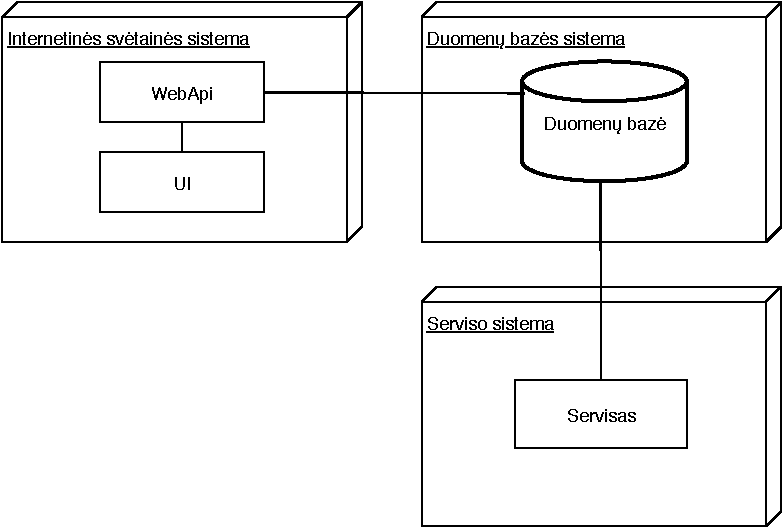
\includegraphics[width=0.9\textwidth]{figs/arch1lt.pdf}
	\caption{Sistemos architektūros schema}
	\label{fig:arch1}
\end{figure}

Sistemos architektūros schemos \ref{fig:arch1} pavyzdyje matome tris sistemas – internetinės svetainės sistemą, duomenų bazės sistemą ir serviso sistemą. Internetinės svetainės sistemoje veikia pati internetinė svetainė, kurioje vyksta prisijungimas prie sistemos, skenavimo užklausų kurimas ir skenavimo ataskaitų parsisiuntimas. Duomenų bazės sistemoje veikia pati duomenų bazė, kurios paskirtis yra laikyti skenavimo užklausas ir jų rezultatus, taip pat laikyti prisijungo duomenis. Serviso sistemoje veikia pats servisas, kuris atlieka visa skenavimo logiką ir visą bendravimą su skenuojama internetine svetaine. Taip pat bendrauja ir su duomenų baze, iš jos pasiima visus duomenis reikalingus skenavimui ir į ją deda visus skenavimo rezultatus. 

UI aplikacija internės svetainės sistemoje sukurta naudojant Angular. WebApi, kuris atsakingas už visą bendravimą su duomenų baze bei skenavimo ataskaitų formavimą, sukurtas naujant ASP.NET Core. 
Duomenų bazė sukurta naudojant Microsoft SQL. Serviso sistemoje esanti serviso aplikacija sukurta naudojant .NET Core, su kuriuo parašyta visa pararelinė skenavimų paleidimo logika ir bendravimas su duomenų baze, Bash scriptus, kurie skirti kurti konteinerius ir vykdyti skenavimus, Docker, kuris skirtas kurti konteinerius ir užtikrinti visos sistemos saugumą ir stabilumą. Visos sistemos naudoja Ubuntu 16.04 operacinę sistemą. 

\subsection{Vartotojo sąsaja}

\begin{figure}[H]
	\centering
	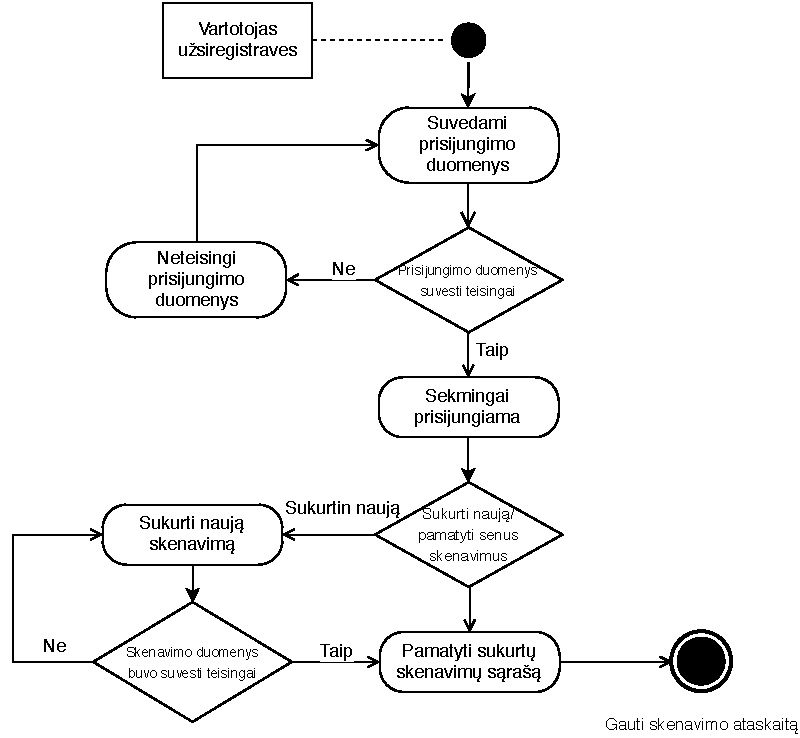
\includegraphics[width=0.9\textwidth]{figs/Activitylt.pdf}
	\caption{Aktyvumo diagrama}
	\label{fig:activity}
\end{figure}

Aktyvumo diagramoje, kuri yra \ref{fig:activity} pavyzdyje, galima matyti visus pasirinkimus, kuriuos vartotojas turi. Vartotojo sąsaja sukurta naudojant Angular, visi atliekami veiksmai keliauja į API, kuris sukurtas su ASP.NET Core. API vyksta visa internetinės svetainės logika – autentifikacijos valdymas bei duomenų valdymas. Jungimosi metu į UI suvedami duomenys keliauja į API, kuriame prisijungimo duomenys yra verifikuojami su duomenų baze. Sėkmingai prisijungus, vartotojas gali arba kurti naują skenavimo užklausą, arba pamatyti jau sukurtas. Kuriant skenavimo užklausą, duomenys taip pat yra tikrinami, patikrinus ir sėkmingai užregistravus skenavimo užklausą, vartotojas gali eiti į skenavimų sąrašą, kur bus pateiktas jo sukurtas skenavimas, ataskaitų parsisiuntimo nuorodos, arba jis gali kurti naują užklausą.

\subsection{Saugios aplinkos užtikrinimas}
\label{sec:safe}

Internetinių svetainių skenavimo įrankyje saugi aplinka užtikrinama naudojant Docker, kuris pasižymi tuo, kad su ja yra kuriami konteineriai, kurie yra įzoliuoti nuo likusios sistemos. Pačią Docker technologiją galima lyginti su virtualiomis mašinomis, kurias pavyzdžiui kuria VirtualBox įrankis. Skirtumas tarp jų  yra didžiulis. Docker konteineriai yra kuriami operacinės sistemos lygyje, skirtingai negu VirtualBox virtualios mašinos, kurios kuriamos geležies lygyje, taip pat kiekviena virtuali mašina turi turėti savo atskirą operacinę sistemą, o konteineriai tiesiog naudoja tą pačią opericinę sitemą, kurioje jie yra kuriami, todėl konteineriai reikalauja žymiai mažiau išteklių, veikia žymiai greičiau, juos galima greitai kurti ir naikinti\cite{merkel2014docker}. Visa tai yra svarbu sistemai, nes kiekvienam procesui yra kuriamas atskirs konteineris, po kiekvieno proceso įgyvendinimo konteineris yra sunaikinamas. Konteineriu greitis leidžia tai padaryti greitai ir saugiai, nėra priežasties, kodėl konteinerius reikėtų pernaudoti, nereikia atskirai surašinėti operacinių sistemų ir jų konfiguruoti, taip pat mažas resursų kiekis nestabdo visos sistemos bendrai ir užtikrina, kad sistema nesustos veikti.

\begin{figure}[H]
	\centering
	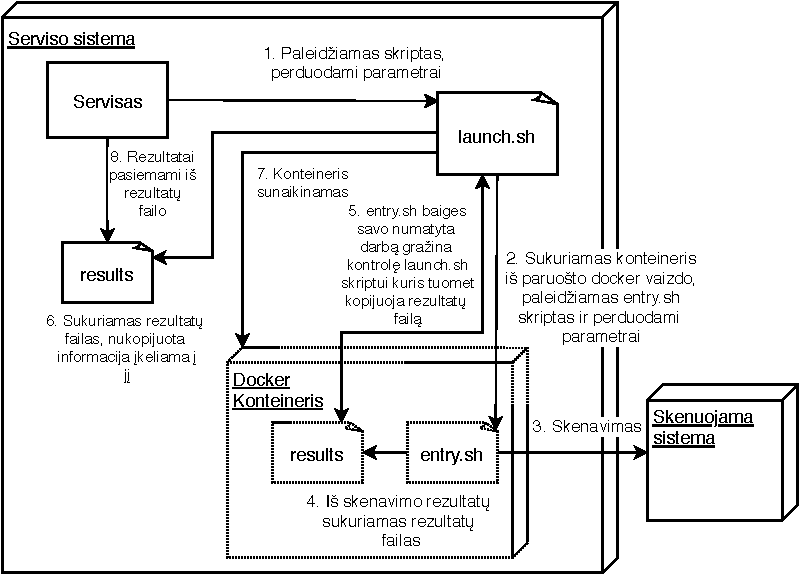
\includegraphics[width=1\textwidth]{figs/docker.pdf}
	\caption{Saugios aplinkos užtikrinimo veikimas}
	\label{fig:docker}
\end{figure}

Pilnoje saugios aplinkos įgyvendinimo schemoje, kuri yra \ref{fig:docker} pavyzdyje, matome visą procesą, kuris užtikrina sistemos ir įrankio saugumą. Kiekvieno žingsnio, kuris yra įgyvendinamas paaiškinimas:
\begin{enumerate}
	\item Iš pradžių servisas paleidžia „launch.sh“ bash skriptą, tuo pačiu skriptui perduodamas parametrus reikalingus skenavimui įgyvendinti. Servisas viso šio skripto metu laukia, kol skriptas pabaigs savo darbą.
	
	\item Skriptas „launch.sh“ sukuria konteinerį pagal pasirinktą docker vaizdą. Kiekvienas atliekamas skenavimas turi savo specifinį vaizdą, kuris yra sukuriamas vieną kartą, ir visą laiką laikomas išsaugotas.
	Kurdamas konteinerį skriptas taip pat į konteinerį perduoda bash komandą, kuri paleidžia „entry.sh“ skriptą ęsanti konteineryje ir paleidimo metu perduoda jam parametrus, kuriuos pats gavo iš serviso. Skriptas konteineryje atsiranda kartu su jo sukurimu, nes šis skriptas taip pat saugomas vaizde. Skriptas „launch.sh“ paleides skriptą „entry.sh“ laukia, kol jis baigs savo darbą.
	
	\item Skriptas „entry.sh“ įgyvendina skenavimo komandas su gautais parametrais iš „launch.sh“ skripto. Jeigu skenavimo metu tenka parsisiųsti failų iš skenuojamos sistemos, šis skriptas taip pat juos parsiunčia ir patalpina į konteinerį. 
	
	\item Skriptas „entry.sh“ įgyvendines skenavimo komandas, sukuria rezultatų failą, į kurį įdeda rezultatus, prireikus juos suformatuoja tam tikra tvarka prieš įdėdamas. Tuomet jis baigia savo darbą.
	
	\item Skriptas „launch.sh“ sulaukes skripto „entry.sh“ pabaigos, kopijuoja rezultatų failą ęsantį konteineryje.
	
	\item Tuomet skriptas „launch.sh“ sukuria failą pagrindinėje sistemoje ir įkelia į jį nukopijuotus duomenis.
	
	\item Skriptas „launch.sh“ sunaikina konteinerį su visais jame esančiai failais ir baigia savo darbą. Jeigu konteineryje buvo atsiųsta failų iš skenuojamos sistemos, jie taip pat yra sunaikinami.
	
	\item Servisas sulaukia skripto „launch.sh“ pabaigos ir toliau vykdo savo darbą, pasiima rezultatus iš rezultatų failo ir juos naudoja tolimesniuose procesuose.
\end{enumerate} 

\subsection{Įgyvendinami skenavimo metodai}

Iš viso yra įgyvendinti keturi skenavimo metodai. Šie metodai aprėpia didelį skaičių potencialių pažeidžiamumų, taip pat su šiais metodais galima aptikti dažniausiai esančius pažeidžiamumus, kurie pasitaiko sistemose. Metodai apima atvejus ne vien tik situacijas, kai esantys pažeidžiamumai yra aptinkami prieš įsilaužimą, bet apima ir įsilaužimo ir po ųsilaužimo situacijas.

\subsubsection{Išorinis sistemos skenavimas}
\label{sec:scanOutside}
Išorinis sistemos skenavimas skirtas tam, kad aptiktų atvirius prievadus, patikrintų, kokią informaciją išduota pati sistema – kokią operacinę sistemą pati sistema naudoja, kokia tos operacinės sistemos versija, kokios aplikacijos ar sistemos veikia toje sistemoje, ar prie šių sistemų galima jungtis, ar gali prisijungti anoniminiai vartotojai. Skenavimo įgyvendinimo metu yra sukuriamas konteineris, iš kurio yra atliekamas skenavimas. Skenavimui pasibaigus yra surenkami rezultatai ir atiduodami servisui, konteineris yra saugiai sunaikinamas, o rezultatai patalpinami į duomenų bazę.
\subsubsection{Failų skenavimas}
\label{sec:scanFile}
Internetinės sistemos failų skevimas skirtas patikrinti ar į sistemą jau nebuvo ųsilaužta, ir joje nėra paliktų kenkėjiškų programų. Šis skenavimas yra įgyvendinimas skenavimo užklausos metu. Sukuriamas Docker konteineris, iš kurio naudojant \textit{FTP} prisijungiama prie sistemos. Iš \textit{FTP} direktorijos yra parsiunčiami visi failai į konteinerį, tuomet yra generuojami visų failų MD5 maišos žodžiai, kurie yra paruošiami tikrinimui ir yra patikrinami žinomų kenkėjiškų programų failų MD5 maišos žodžių duomenų bazėje. Tuomet rezultatai yra gražinami į servisą, o pats konteineris yra saugiai sunaikinamas. Rezultatai patalpinami į duomenų bazę.
\subsubsection{Internetinės svetainės prieigos skenavimas}
\label{sec:scanUrl}
Internetinės svetainės prieigos skenavimas yra skirtas tam, kad aptiktų potencialias \textit{MITM} atakas, fišingo svetaines, kenkėjiškų programų svetaines. Veikimas yra toks, kad svetainės adresas yra nusiunčiamas trečiajai šaliai, kuri svetainės adresą skenuoja su įvairiomis antivirusinėmis. Tuomet yra pateikiama detali ataskaita. Kadangi šio skenavimo metu nėra kontaktuojama su pačia svetaine tiesiogiai, Docker konteineriai nėra kuriami.
\subsubsection{Internetinės svetainės enumeravimas}
\label{sec:scanEnum}
Internetinės svetainės enumeravimas yra skirtas tam, kad aptiktų potencialias internetinės svetainės spragas, tokias kaip atviras direktorijas, kuriose puolėjas gali be jokių kliūčių perskaityti jose ęsančių failų turinį. Taip pat aptinkama visi internetinės svetainės puslapiai, prie kurių vartotojas gali prieiti be jokios autentifikacijos, sakykime prie administratoriaus puslapio, šios problemos kyla dėl blogai sukonfiguruotų teisių ar pačio puslapio autentifikacijos. Skenavimo metu yra sukuriamas konteineris, kuriame vykdomas enumeravimas, konteineryje susigeneruoja rezultatų failas, kuris yra gražinamas servisui, o pats konteineris yra saugiai sunaikinamas. Rezultatai yra patalpinami į duomenų bazę.

\subsection{Skenavimo užklausų įgyvendinimas}
\label{sec:allProc}

Skenavimo užklausų įgyvendinimas yra svarbiausias procesas šiame įrankyje. Skyriuje \ref{sec:allProc} bus paaiškinama visas skenavimo užklausos įgyvendinimas nuo jos sukurimo iki skenavimo užklausos ataskaitos parsisiuntimo.

\begin{figure}[H]
	\centering
	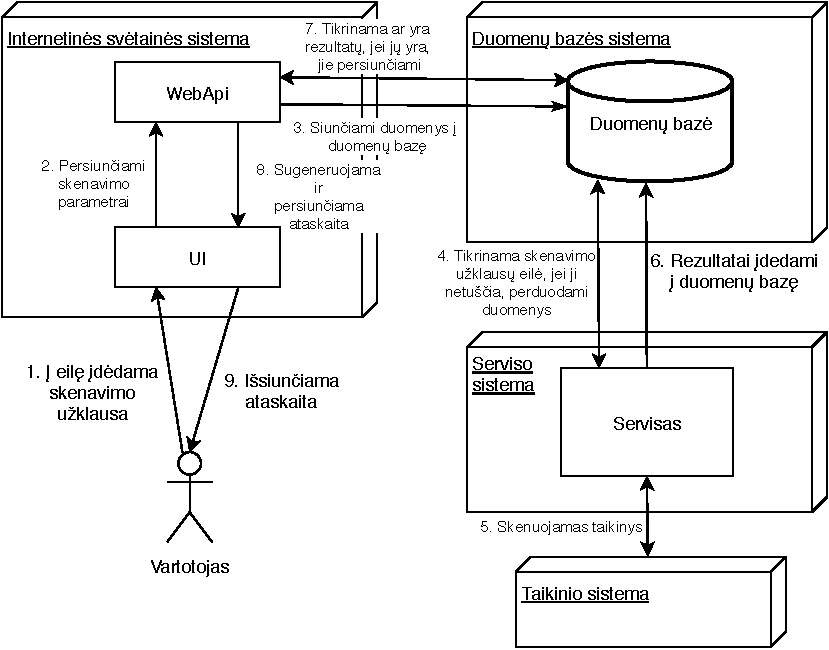
\includegraphics[width=1\textwidth]{figs/Fulllt.pdf}
	\caption{Įrankio veikimo schema}
	\label{fig:full}
\end{figure}

Įrankio veikimo schemoje, kuri yra \ref{fig:full} pavyzdyje, galima matyti daug procesų, kurie veikia paeiliui arba paraleliai. Kiekvieno proceso paaiškinamas paeiliui:

\begin{enumerate}
	
	\item Prisijungęs vartotojas kurdamas skenavimo užklausą suvedada atitinkamus parametrus tokius kaip: Internetinės svėtainės adresą, FTP atrasą, FTP prisijungimo duomenis;
	
	\item Duomenys yra siunčiami į WebApi, kuriame vyksta visa duomenų verifikavimo logika, tikrinama ar duomenis yra geri, ar adresai yra teisingai suvesti;
	
	\item Verifikuoti duomenys yra siunčiami į duomenų bazę, ir yra išsaugomi;
	
	\item Servise veikia laikmatis, kuris praėjus tam tikram laikui vis tikra ar duomenų bazėje nėra skenavimo užklausų, kurios dar nebuvo įgyvendintos. Jei tokių užklausų yra, duomenys yra paimami;
	
	\item  Pradedama vykdyti skenavimo logika kiekvienai užklausai paeiliui. Užklausos vykdomos paeiliui, o ne iš karto visos tam, kad būtų užtikrintas sistemos stabilumas ir minimalus resursų naudojimas. Jeigu vienu metu būtų įgyvendinamos šimtai užklausų, rizikuojama, kad sistema pritrūks resursų visoms operacijoms įgyvendinti. Nors ir kiekviena užklausa įgyvendinama paeiliui, bet kiekvienai užklaisai skenavimo operacijos yra vykdomomos paraleliai. Šiuo atveju nėra rizikuojama, kad sistema pritrūks resursų, nes yra vykdomas fiksuotas skaičius operacijų;
	
	\item Baigusis operacijoms rezultatai yra formatuojami ir įdedami į duomenų bazę.
	
	\item Tuo tarpu WebApi vykdo užklausas į duomenų bazę ar dar nėra skenavimo užklausos duomenų kiekvieną kartą, kai vartotojas perkrauna puslapį, kuriame yra skenavimo užklausų sąrašas, gavus atsaką, kad duomenų yra, vartotojui leidžiama atsisiųsti ataskaitą;
	
	\item Vartotojas pateikia užklausą gauti skenavimo užklausos ataskaitą. Tuo metu paimami duomenys iš duomenų bazės ir yra generuojama ataskaita HTML formatu. Sugeneruojamas parsisiuntimo adresas.
	
	\item Vartotojui leidžiama parsisiųsti ataskaitą.
	
\end{enumerate}

\begin{figure}[H]
	\centering
	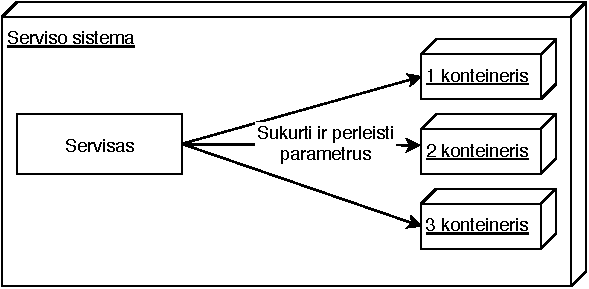
\includegraphics[width=0.9\textwidth]{figs/1Containerlt.pdf}
	\caption{Konteinerių sukurimas įgyvendinant skenavimo užklausas}
	\label{fig:1Container}
\end{figure}

Serviso sistemoje įgyvendinant skenavimo užklausas yra kuriami trys docker konteineriai kaip pavaizduota \ref{fig:1Container} pavyzdyje. Apie patį konteinerių kurimo procesą buvo rašyta \ref{sec:safe} skyriuje. Kiekvieno konteinerio procesas reikalauja skirtingų parametrų, nes atlieka skirtingus darbus. Jie gaunami \ref{fig:full} pavyzdžio pirmajame punkte.

\begin{figure}[H]
	\centering
	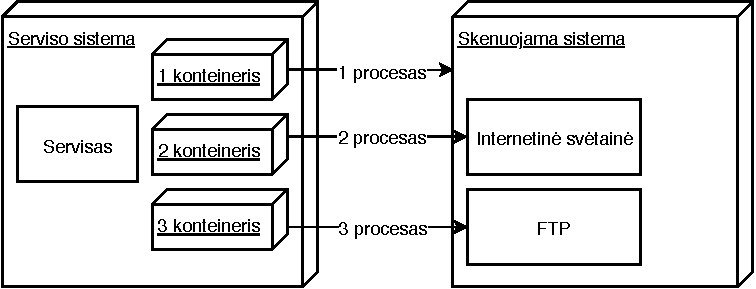
\includegraphics[width=0.9\textwidth]{figs/2Containerlt.pdf}
	\caption{Proceso Veikimas}
	\label{fig:2Container}
\end{figure}

Proceso veikimas pavaizduotas \ref{fig:2Container} pavyzdyje ir jame matome, kad visi konteineriai atlieka skirtingus procesus paraleliai, pirmasis konteineris atlieka skenuojamos sistemos išorinę analizę, apie kurią daugiau buvo rašyta \ref{sec:scanOutside} skyriuje, šiam konteineriui kaip parametras yra paduodamas sistemos IP adresas. Antrasis konteineris atlieka skenuojamos internetinės svetainės enumeraciją, kuri aprašyta \ref{sec:scanEnum}, šiam konteineriui kaip parametras yra paduodamas internetinės svetainės adresas. Trečiasis konteineris jungiasi į prie serverio naudodamas FTP protokolą ir atlieka failų skenavimą, kuris aprašytas \ref{sec:scanFile} skyriuje, šiam konteineriui per parametrus yra paduodi FTP prisijungimo duomenys bei FTP adresas. Taip pat yra įgyvendinamas ir internetinės prieigos skenavimas, kuris aprašytas \ref{sec:scanUrl} skyriuje, tačiau šiam skenavimui nereikalinga skenuojamos sistemos prieiga, todėl konteineris jam nėra kuriamas.

\begin{figure}[H]
	\centering
	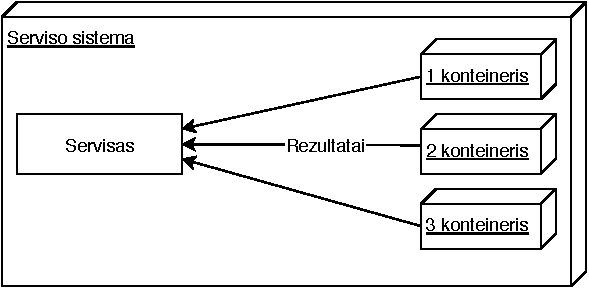
\includegraphics[width=0.9\textwidth]{figs/3Containerlt.pdf}
	\caption{Rezultatų gražinimas}
	\label{fig:3Container}
\end{figure}

Įgyvendinus visus skenavimo procesus, rezultatai yra gražinami pačiam servisui, o patys konteineriai susinaikina. Taip pat internetinės svetainės prieigos skenavimo rezultatai yra pasiimami ir perduodami servisui, servisas vėliau juos formatuoja ir talpina į duomenų bazę. Pats duomenų perdavimas ir konteinerių sunaikinimas yra aprašytas \ref{sec:safe} skyriuje.


\subsection{Įrankio skenavimo metodų platforma}

Įrankis yra puikiai pritaikytas naudoti bet kokioje sistemoje, taip pat jį ypač patogu pritaikyti bet kokiame scenarijuje. Šis įrankis yra plačiai naudojamas kibernetinio saugumo bendruomeneje ir taip pat yra ypač efektyvus atliekant tinklo skanavimus ar analizę. Atsisžvelgus į šiuos faktus, šis įrankis tampa butinybė bet kokioje spragų skanavimo sistemoje dėl savo didelio potencialo ir bendruomenės pasitikėjimo.
\begin{algorithm}
	\caption{Įrankio platformos pseudo kodas}
	\label{alg:pseudo}
	\begin{algorithmic}
		\STATE $ScanRequests \gets Database$
		\IF{$ScanRequests > 0$}
		\FORALL {$ScanRequests$}
		\STATE $ThreadPool \gets Scan1(ScanRequest)$
		\STATE $ThreadPool \gets Scan2(ScanRequest)$
		\STATE $ThreadPool \gets Scan3(ScanRequest)$
		\STATE $ThreadPool \gets Scan4(ScanRequest)$
		\STATE $ThreadPool. Wait For All$
		\ENDFOR
		\STATE $Database \gets ThreadPool.Results$
		\ENDIF
	\end{algorithmic}
\end{algorithm}


Įrankio kurimo metu buvo sukurta platforma, kuri yra integruota į patį įranki. Platforma yra skirta lengvai pridėti naujus skenavimo būdus ir funkcijas. Iš šios platformos yra startuojami visi jau esantis skenavimo metodai. Naujų skenavimo metodu pridėjimas vyksta programiškai, bet pati platforma parašyta taip, kad norint pridėti kažka naujo, nereikia programuoti visko iš naujo. Šios platformos kodą galime matyti \ref{alg:pseudo} algoritme. Iš pradžių pasiimame visas skenavimo užklausas, kurios dar nebuvo vykdytos iš duomenų bazės, tuomet iteruojame per kiekviena iš jų ir parareliai paleidžiame visus skenavimo metodus. Kai visi skenavimo metodai yra paleisti, laukiame, kol visi jie pasibaigs. Visiems skenavimams pasibaigus, resultatus patalpiname į duomenų bazę.


\subsection{Aptiktini pažeidžiamumai}

Šiuo metu skenavimo įrankis gali aptikti šiuo pažeidžiamumus:
\begin{itemize}
	\item Aptiktinos yra \textit{MITM} atakos tikrinant internetinės svetainės atsakus;
	\item Aptinkama ar puslapis yra nesaugus naudoti ir turi kenkėjiškų programų;
	\item Aptiktinos direktorijos, kurios sąrašo pavidalu gražina savo turinį, taip atsitinka dėl neteisingai sudėtų teisių sistemoje, dėl šio pažeidžiamumo puolėjas atradęs šią direktoriją gali be jokių kliūčių peržiūrėti joje esančius failus;
	\item Aptiktini puslapiai, prie kurių neprisijungęs vartotojas neturėtų galimybės prieiti. Kaip pavyzdį galima būtų pateikti prisijungimo vietas prie administratoriaus sąsajos;
	\item Aptiktinkamos kenkėjiškos programos ir infekuoti failai;
	\item Aptinkamos sistemos, kurios veikia skenuojamoje sistemoje;
	\item Aptinkami atidaryti prievadai.
\end{itemize}

\subsection{Įgyvendinti uždaviniai}
\label{sec:example}
Įgyvendinti šie apsibrėžti uždaviniai: 
\begin{itemize}
	\item Sukurta svetainė, kuri leidžia vartotojui kurti skenavimo užklausas ir po jų sukurimo leidžia atsisiųsti suformatuotus rezultatus;
	\item Sukurta platforma ir paruoštukai, kurie leidžia lengvai pridėti naujus skenavimo metodus į įrankį;
	\item Sukurta saugi aplinka, kuri leidžia vartotojui saugiai skenuoti sistemas ir jų failus, nesibaiminant infekuoti pačio įrankio sistemos;
	\item Aptinkami pažeidžiamumai ir pati sistema paruošta naudojimui;
	\item Sugeneruojama ir pateikiama ataskaika, kurią lengva suprasti vartotojui.
\end{itemize}


\subsection{Trūkumai}
\label{sec:example}

Įrankio kurimo procesas yra ypač sudėtingas dėl didelio skaičiaus skirtingų technologijų, su kuriomis yra kuriamos internetinės svetainės, taip pat kiekviena internetinė svetainė skiriasi nuo kitų savo sistemos komponentais, architektūra, naudojamomis technologijomis.

Kurimo metu buvo planuota panaudoti trečios šalies įrankį SqlMap. Šio įrankio paskirtis yra ieškoti ar internetinė svetainė yra pažeidžiama SQL injekcijos atakoms. Tokio tipo skenavimui reikėtų sukurti internetinės svetaines puslapių kodo funkciją, kuri svetainės puslapyje ieško dinaminių nuorodų. Šios nuorodos priema parametrus savo nuorodose. Tuomet SqlMap įrankis bando į šiuos parametrus įdėti manipuliuotą tekstą, kuris įvykdytų užklausą duomenų bazeje. Šio įrankio funkcionalumo įgyvendinimas šioje skenavimo sistemoje tapo perdaug problematiškas ir laiko užimantis dėl pačios funkcijos, kuri ieškotų tokių įveščių internetinėje svetainėje. Dėl šios priežasties SqlMap funkcionalumo atsisakyta.

Kurimo metu taip pat buvo užsibrėžta įgyvendinti statinę analizę. Šis tikslas buvo įgyvendintas nepilnai, patys failai buvo tikrinami žinomų kenkėjiškų programų duomenų bazėje, bet internetinės svetainės kodas nebuvo tikrinamas. Šio tikslo atsisakyta ir statinės analizės technikų įgyvendinimai perkelti į ateities darbus. Šio atsisakymo priežastis yra ta, kad kiekvienai programavimo kalbai reikalingas atskiras statinės analizės įgyvendinimas, kieviena kalba yra kitokia, jos funkcionalumas ir sintaksė pat pat, dėl šios priežasties tokio funkcionalumo kurimo kaštai stipriai didėja.


 %Conclusions section
 
 \sectionWithoutNumber{Rezultatai}{}
 
 Sukurtas saugus pažeidžiamumų skaitytuvas sistemų auditavimui naudojantis naujausiomis technologijos. Pažeidžiamumų skaitytuvas yra modulinis, turi tris modulius: Internetinę svetainę, duomenų bazę ir servisą, kuris atlieka visus skenavimus. Visos trys dalys geba veikti atskirai, taip pridedant papildomą saugumo ir stabilumo sluoksnį.
 
 Pats skaitytuvas įgyvendina keturis skirtingus skenavimus skirtingiems pažeidžiamumams aptikti. Skaitytuvas geba aptikti išorinius pažeidžiamumus skenuodamas sistomos išorė, taip bandydamas aptikti atidarytus prievadus, sistemos operacinę sistema bei jos versiją, veikiančias kitas sistemas, jų tipus ir versijas pagrindinėje sistemoje, tokias kaip: duomenų bazę, internetines svetaines. Taip pat yra bandoma aptikti, kokiais protokolais galima prisijungti prie duomenų bazės ir ištestuoti, ar galima prie jų jungtis anonimiškai. Skaitytuvas taip pat geba jungtis prie sistemos per FTP, prisijungus parsisiųsti visus failus ęsančius joje ir tikrinti ar jie egzistuoja žinomų kenkėjiškų programų duomenų bazėje. Skaitytuvas gali tikrinti internetinę svetainę, kuri veikia pasirinktoje sistemoje, tikrinama ar ši svetainė turi direktorijų, kurios pateikia savo turinio sąrašą, tokiose direktorijose failų turinį gali skaityti bet kas, taip randant neteisingai sudeliotas teises sistemoje. Taip pat ieškoma ir puslapių sąrašo, kurį neautentifikuotas vartotojas gali pasiekti, taip bandoma surasti puslapius, prie kurių vartotojas gali prieiti, bandoma surasti, ar yra prieigos taškų, kurie neturėtu būti prieinami kiekvienam. Taip pat yra tikrinama ir pati prieiga prie internetinės svetainės, bandoma rasti ar nėra vykdoma MITM ataka ir ar internetinėje svetainėje neveikia kenkėjiškos programos. 
 
 Skaitytuvo saugumas yra užtikrinamas naudojant docker konteinerius. Parašyti specialiūs paruoštukai kiekvienam skenavimui, kurie leidžia sukurti specifinį konteinerį. Naudojant konteinerių technologiją yra pasiekiamas saugumas, kuris apsaugo skaitytuvo sistemą nuo potencialių grėsmių, kurios gali slėptis internetinėje svetainėje. Kiekvieno skenavimo užklausa vykdoma paraleliai paleižiant skenavimus, o tai užtikrina didesnį greitį. Skenavimo rezultatai keliauja į duomenų bazę, iš kurios vėliau yra paemami formuoti ataskaitą. Ataskaita yra specializuota kiekvienam testui.
 
 Internetinė svetainė veikia atskirai nuo visos likusios skaitytuvo struktūros ir yra skirta tik bendrauti su vartotoju. Svetainėje yra autentifikacija, kuri reikalinga kuriant naujas skenavimo užklausas. Svetainėje galima kurti naujas skenavimo užklausas, peržiurėti visas kitas, ir parsisiųsti jų visų ataskaitas. 
 
\sectionWithoutNumber{\keyWordConclusions}{conclu}

Išvados bei rekomendacijos.


%ateities darbų gairės, planas/next steps of the work
\sectionWithoutNumber{Ateities darbų planas}{future}

Ateities darbų plano gairės:

\begin{itemize}
	\item Įgyvendinti statinę analizę, parsisiuntus internetinės svetainės kodą, jį analizuoti priklausomai nuo to, kokia kalba jis parašytas;
	\item Įgyvendinti svetainės dinaminę analizę, parsisiuntus internetinę svetainę, automatizuoti jos paleidimą ir paleidus įgyvendinti dinaminę analizę.
	\item Įgyvendinti vidinių pažeidžiamumų skenavimą, prisijungti prie sistemos naudojans SSH, paleisti scriptus, kurie randa sistemos spragas.
\end{itemize}


 %file References.bib
\referenceSources{References}
%\bibliographystyle{ieeetr}

%% this part is optional
%%\newpage
%%\begin{appendices}


%%\end{appendices}


\end{document}
